\documentclass[11pt,prd,letterpaper,amsmath,amssymb,final,nofootinbib
%linenumbers 
,unsortedaddress,superscriptaddress
]{revtex4-1}
% Fun and exciting LaTeX packages!

\pdfoutput=1

%Margins
\usepackage[top=0.9in, bottom=0.9in, left = 0.9in, right=0.9in]{geometry}

\usepackage{graphicx}% Include figure files 
%\usepackage{subfig}
%\usepackage{caption}
%\usepackage{subcaption}
\usepackage{dcolumn}% Align table columns on decimal point
\usepackage{bbm}% blackboard bold
\usepackage{textcomp}% I can't remember what this one does...
\usepackage{color}% Change font colors
\usepackage{gensymb}% Some nice math symbols...
\usepackage{wasysym}
\usepackage{amssymb}
\usepackage{enumerate}
\usepackage{geometry}
\usepackage{setspace}
%\usepackage{hyperref}
%\usepackage{lineno}
\setcounter{tocdepth}{3}

  
%\linenumbers
% Begin main document...
\begin{document}

\title{ THEIA: \\ {\small }}

\author{THEIA Collaboration}
\affiliation{Many and Varied}

\maketitle

\section*{Executive Summary}

\newpage

\tableofcontents
\setcounter{tocdepth}{5}
\newpage

\section{Introduction and THEIA Overview - GDOG, Bob, JRK, Michi}

Standard intro

Include description of phased deployment

e.g. refer to THEIA-i, THEIA-ii, THEIA-iii

Define the baseline design for each here, so that physics sections can simply refer back

e.g. THEIA-ii might be 50ktonne 10\% WbLS, 90\% coverage

whereas THEIA-iii might be the above with 5\% WbLS but a bag containing LS + Te/Xe

\section{Technology Developments}
\subsection{Water-based Liquid Scintillator - R. Svoboda}

\subsection{Photon Sensors - \bf volunteers?}
\subsection{Reconstruction Techniques -- B. Wonsak \& M. Tsanov}
%Including techniques and results (to date) for both low and high energy events


% DOCUMENT BEGIN
%==================================================================================================%
%\documentclass[a4paper,11pt]{article}
%==================================================================================================%

% PACKAGES
%==================================================================================================%

%\usepackage[utf8]{inputenc}	%UTF8 file encoding
%\usepackage[lmargin=3cm,rmargin=4cm,tmargin=3.5cm,bmargin=3.5cm]{geometry}
%
%\usepackage[T1]{fontenc}
%% \usepackage{lmodern}
%% \usepackage{scrextend}
%\usepackage{amssymb,amsmath}
%%\usepackage{graphicx, amsthm, multirow}
%\usepackage{graphicx, amsthm}
%\usepackage{mathrsfs}
%% \usepackage[outdir=../images/eps/]{epstopdf}
%% \usepackage{cite}
%% \usepackage{url}
%
%% \usepackage[margin=12pt,font=small,labelfont=bf,labelsep=endash]{caption}
%\usepackage{subcaption}
%\usepackage{color}
%% \usepackage{todonotes}
%% \usepackage{siunitx}
%% \usepackage{textcomp}
%\usepackage{lineno}
% \usepackage{multirow}
% \usepackage[utf8]{inputenc}
% %\usepackage[doublespacing]{setspace}
% \usepackage[printonlyused,nohyperlinks]{acronym}
% \usepackage{microtype}
% \usepackage[english,german]{babel}
% \usepackage{array}
% \usepackage{pbox}
% \usepackage[hang,flushmargin,multiple,splitrule]{footmisc} 
% \usepackage{enumitem}
% 
% \usepackage[parfill]{parskip}
% \usepackage{titlesec}
% 
% \titlespacing\chapter{0pt}{0pt plus 1pt minus 1pt}{10pt plus 2pt minus 2pt}
% \titlespacing\section{0pt}{12pt plus 4pt minus 2pt}{4pt plus 1pt minus 1pt}
% \titlespacing\subsection{0pt}{12pt plus 4pt minus 2pt}{4pt plus 1pt minus 1pt}
% \titlespacing\subsubsection{0pt}{12pt plus 4pt minus 2pt}{4pt plus 1pt minus 1pt}
% 
% 
% \usepackage[hyperfootnotes=false]{hyperref}
% \hypersetup{
%     colorlinks,
%     citecolor=black,
%     filecolor=black,
%     linkcolor=black,
%     urlcolor=black
% }
% \usepackage[all]{hypcap}

% DOCUMENT CONFIG
%==================================================================================================%
%
%\title{Reconstruction}
%\author{}
%\date{\today}
%
%
%% Load custom commands, acronyms and abbreviations
%%\input{TexCommands.tex}
%%\input{AcronymsAndAbbreviations.tex}
%
%% DOCUMENT BEGIN
%%==================================================================================================%
%\begin{document}
%%==================================================================================================%
%
%\maketitle
%%\pagenumbering{Roman} % roman numbers before the introduction
%% ABSTRACT
%%__________________________________________________________________________________________________%
%%\begin{abstract}
%%Here will be an abstract...
%%\end{abstract}
%%__________________________________________________________________________________________________%
%
%\tableofcontents % table of contents
%\pagenumbering{arabic} % change to arabic numbers

% SECTIONS
%__________________________________________________________________________________________________%

\newpage

\vfill

%\section{Reconstruction}


While in the past Cherenkov detectors have been very successful in reconstructing various properties of the particles involved
in a neutrino event, liquid scintillation detectors have long been thought as a source for calorimetric information only. 
However, in recent years it became obvious that the time information of the light in liquid scintillators can be used to 
access a wide range of information, similar or even superior to what a pure Cherenkov detector can deliver. 

Basically, there are two complementary approaches to reconstruction in both detector types and consequently also in WBLS 
detectors. The first approach developed in MiniBooNE\cite{patt09} and successfully applied in T2K\cite{Abe:2015awa} follows a likelihood ansatz to 
find the optimal track parameters and compare different hypotheses. In contrast to this, the three-dimensional topological 
reconstruction tries to picture the spatial distribution of the energy deposition within the detector without using a 
specific hypothesis. This technique has been developed for the LENA\cite{Wurm:2011zn} detector and also been implemented for the JUNO detector \cite{An:2015jdp}.
These are liquid scintillator detectors, but the application to Cherenkov detectors is straight forward. 

Both methods have been improved considerably over the last couple of years. For example fitQun, the reconstruction software 
used by T2K is now able to reconstruct up to 6 Cherenkov rings. This alone will increase the expected sensitivity 
for example for CP-violation in the LBNF beam significantly in comparison to previous studies like \cite{Goon:2012if}. In addition, the 
topological reconstruction promises large volume liquid detectors the same capabilities as only highly segmented detectors 
used to have (with all the implications of that). This includes possibilities for particle identification at energies as low as
a few MeV based on topological information. This ability will be further enhanced by the combination of the two light species,
Cherenkov and scintillation light, as can be seen in \cite{Elagin:2016zgp}, where Cherenkov-Scintillation separation is used to
identify the two electrons of a 0$\nu\beta\beta$-decay.

To give an overview on the state of the art in reconstruction, this section is divided into three subsections. The first
subsection is dedicated to the likelihood approach and its latest results. The second subsection describes the topological 
reconstruction. And the third subsection is dedicated to applications of Cherenkov-light-Separation at low energies.

\subsubsection{Likelihood}

This subsection summarizes the main features of the reconstruction 
method developed for the MiniBooNE detector\cite{patt09}. In this 
method a likelihood function is evaluated for a particle (particles) of some type
with initial kintmatic parameters to have produced the observed collection 
of PMT hits, charges and times, in an event. A key ingredient 
of the likelihood calculation is the predicted hit distribution which 
represents the average response of the detector for such a particle and
therefore the likelihood is a function of the paricle's kinematic parameters. 
The optimal parameters would provide the best agreement between
the predicted and observed hit distributions i.e. the likelihood
function will be at a maximum.

Realistic model of detector response is required to develop a
successful and efficient event reconstruction and identification algorithms.
This requires both {\it in-situ} and {\it ex-situ} measurements
of various optical properties of the water, PMTs and the reflection
of all surface inside the detector. Absorption, scattering, reflections
and fluorescence processes can affect the reconstruction.
In order to account for these effects in the reconstruction,
these optical properties have to be obtained if unknown. 

Single track is parametrized with 7 parameters: starting point $(x_0, y_0, z_0)$,
starting time $t_0$, direction $\theta_0, \phi_0$ with respect to the beam
and kinetic energy $E_0$. We refer to this vector as ${\bf u}$.
Track information is obtained by maximizing the likelihood that
track with vector ${\bf u}$ will produce the observed PMT
measurements. The likelihood for an event assuming all PMTs are independent
is given by

\begin{equation}
	L({\bf q, t; u})=\prod_i^{N_{unhit}} P_i(\text{unhit}; {\bf u})\times\prod_j^{N_{hit}} P_j(\text{hit}; {\bf u})f_q(q_j;{\bf u}) f_t(t_j;{\bf u}).
\end{equation}
Here $P_i(\text{unhit}; {\bf u})$ is the probability PMT $i$ is not hit given ${\bf u}$,
$P_i(\text{hit}; {\bf u})$ is the probability PMT $i$ is hit given ${\bf u}$,
$f_q(q_j;{\bf u})$ is the probability density function for the measured charge $q$ given ${\bf u}$ and
predicted charge $q_j$,
$f_t(t_j;{\bf u})$ is the probability density function for the measured time $t$ given ${\bf u}$
evaluated time $t_j$. Product is carried over all PMTs. For convenience 
we can work with the negative logarithm of the likelihood which can 
be written as a sum of negative logarithms. We will use $F_q$ and $F_t$ to denote the
charge and the time negative logarithm likelihoods respectively  
\begin{equation}
	-\log L({\bf u}) \equiv F_q({\bf u}) + F_t({\bf u}),
\end{equation}

\begin{equation}
	F_t({\bf u}) = -\sum_i^{N_{hit}} \log f_t(t_i;{\bf u}),
\end{equation}

\begin{equation}
	F_q({\bf u}) = -\sum_i^{N_{unhit}}\log P_i(\text{unhit}; {\bf u})-\sum_i^{N_{hit}}\log P_i(\text{hit}; {\bf u}) - \sum_i^{N_{hit}} \log f_q(q_i;{\bf u}).
\end{equation}
From here on we will refer to $F_q$ and $F_t$ simply as the charge and the time likelihoods.

If the number of observed photoelectrons (PE), $n_i$, is known for a given PMT one can assume
that $f_q(q_i;{\bf u})$ is fully specified regardless of detector properties.
In addition, $n_i$ can be assumed to be Poisson distributed with a mean value
$\mu_i({\bf u})$ (predicted charge) for which the notation $\mu_i$ will be
used with implicit dependence on ${\bf u}$. As a result, the probability
for a PMT to have no hit is
\begin{equation}
	P_i(\text{unhit}; {\bf u})\equiv\overline P_i(\mu_i)=e^{-\mu_i}.
\end{equation}
Hence, the probability a PMT has recorded a hit is
\begin{equation}
	P_i(\text{hit}; {\bf u})\equiv P_i(\mu_i)=1-\overline P_i(\mu_i).
\end{equation}
The next step is to separate the predicted charge into prompt and late predicted charge
\begin{equation}
	\mu_i \equiv \mu_{prompt,i} + \mu_{late,i}.
\end{equation}
The prompt predicted charge is a result of \v{C}erenkov light, while the
late predicted charge has contributions from direct \v{C}erenkov light and
indirect light. Sources of indirect light are reflections, scattering and 
fluorescence.

Time PDFs $f_t(t_i;{\bf u})$ depend on the first photon to fire
the PMT. Dependence on ${\bf u}$ can be reduced by introducing
corrected time
\begin{equation}
	t_{cor,i}=t_i-t_0-\frac{r_{mid,i}(E_0)}{c_n}-\frac{\Delta s_{mid}(E_0)}{c},
\end{equation}
where $t_i$ is the measured PMT time, $t_0$ is the measured start time,
$\Delta s_{mid}(E_0)$ is the distance from the track start point to
the mean \v{C}erenkov emission point, $r_{mid,i}(E_0)$ is the distance
from the mean \v{C}erenkov emission point to the PMT, $c_n$ and $c$ are
the speeds of light in water and vacuum respectively. 
Due to the latency period PMT can register only one hit for a given track.
Probabilities of no prompt PEs and no late PEs can be written as
$P(\text{no prompt PEs}) = e^{-\mu_{prompt}}$ and $P(\text{no late PEs}) = e^{-\mu_{late}}$ 
respectively. The probability that a hit contains at least one prompt PE is
\begin{equation}
	w_p=P(\text{prompt PE present}|hit) =\frac{1-P(\text{no prompt PEs})}{1-P(\text{no prompt PEs})P(\text{no late PEs})}.
\end{equation}
This is the weight for the prompt primitive distribution $G_{ch}(t_c,E_0,\mu_{prompt})$, while the $w_l=1-w_p$ is the
weight for the late primitive distribution $G_{late}(t_c,E_0,\mu_{late})$. Finally, the time PDF is
obtained from
\begin{equation}
	f_t(t;E_0,\mu_{prompt},\mu_{late})=w_p G_{ch}(t_c,E_0,\mu_{prompt})+w_l G_{late}(t_c,E_0,\mu_{late}).
\end{equation}
The primitives distribution are created by generating particles throughout the detector in
special runs (e.g. only \v{C}erenkov light and no scattering) and the response is parametrized. 

\subsubsection{3D topological reconstruction}

In this subsection a reconstruction method is presented which aims to provide a 3D topological representation of the energy 
deposition of an event. The method has already been described in detail in \cite{Wonsak:2018uby}. Thus, here only a short description of the
basic concepts is given.

\paragraph{Basic idea}

The general idea of this method is to use the timing information of all registered signals for the construction of isochronal surfaces around each 
  light sensor defined by the signal time. The overlap of these surfaces then indicates likely points of origin of the detected photons 
  and thus can reflect the spatial distribution of the energy deposition of an event. The only assumptions made within this method are 
  that a reference point on the topology is known reasonably well in space and time (the time of the energy deposition) and that all 
  particles propagate through this point in approximately straight lines with the speed of light. The necessary reference point has to be
  provided by a prior analysis of the event. For the sake of simplicity we assume in the following that it is the primary 
vertex of the event. The isochrones can then be described by 


 \begin{equation}
   \label{Eq:Drop-like_shape}
  c \cdot t_{signal} = \abs{|\overline{VX}|} + n \cdot \abs{|\overline{XP}|} \; ,
 \end{equation}
 
 where
  %the signal time $t_{signal}$ is the time between the first interaction at the vertex $V$ and the arrival of an optical photon at a PMT $P$, 
  $n$ is the effective refraction index for the scintillation light, $\abs{|\overline{VX}|}$ is the distance between the vertex $V$ of 
  the event and the point of photon emission $X$, while $\abs{|\overline{XP}|}$ is the distance between the point $X$ and the PMT $P$. 
  
  %This formula describes surfaces which have a drop-like shape as indicated by the black line 
  %in Fig. \ref{fig:SmearedDropShape}.
  
  These isochrones need to be smeared out using a time profile $F(t)$ given by the scintillator 
  properties as well as the time resolution of the optical sensors used. This results in a probability density distribution for each signal.
  Furthermore, the position dependend light detection efficiencies of the PMT have to be taken into account as well as detector effects leading to different 
  light emission in different regions (e.g. a buffer region). We combine these light distribution effects in the function $LD(\vec{x})$.
  
  %Adding these light distribution effects  ($LD(\vec{x})$) substantially modifies 
  %the probability density distribution as can be seen on the right side of Fig.\ref{fig:SmearedDropShape}.
  
  The full topological image of the event is then generated by adding up the individual probability density distribution $P_i(\vec{x})$:
  
   \begin{equation}
  %  \langle N_{photons} \rangle =  % nicht richtig, da man dazu ueber das Volumen integrieren muss
     P(\vec{x})_{total} = \sum_{i} P_i(\vec{x}) = \sum_{i} \left[ \frac{F_i(t(\vec{x})) \cdot LD_i(\vec{x})}{\iiint F_i(t(\vec{x})) \cdot LD_i(\vec{x})  \cdot d\vec{x}} \right] \; .
     \label{eq:TotalP}
  \end{equation}
  %
  
  Here, the index $i$ indicates the individual signals. Thus the $F_i(t(\vec{x}))$ have to be evaluated with the individual signal times $t_{signal, i}$ 
  and the position $P_i$ of the PMT which detected the signal (see equation \ref{Eq:Time_distribution}), while $LD_i$ is an attribute of this PMT depending on its position, 
  optics and sensitivity.   
  
  \begin{equation}
    \label{Eq:Time_distribution}
    F_i(t(\vec{x})) = F_i\left( (\abs{|\overline{VX}|} + n \cdot \abs{|\overline{XP}|_i})/c \right) \; .
  \end{equation}
  
  The result is a 3d map of the expected mean number of detected photons $\langle N_{D}(\vec{x}) \rangle$ coming from a given point. However, to get an impression of the energy
  deposition for a given event, the number of photons emitted from that point $\langle N_{E}(\vec{x}) \rangle$ is deciding.
  Therefore, every point of the 3d distribution has to be weighted by the inverse of the total signal detection efficiency $\eta(\vec{x})$ at that point:
  
  \begin{equation}
     \langle N_{E}(\vec{x}) \rangle = \frac{\langle N_{D}(\vec{x}) \rangle}{\eta(\vec{x})} = \frac{P(\vec{x})_{total}}{\sum_{PMT} LD_{PMT}(\vec{x})}
  \end{equation}
  
  
  In principle, the reconstruction is completed at this stage. However, due to the large width of the time distribution of the individual signals, the picture may not seem very
  sharp. On the other hand, the large number of photons involved still generates a very good spatial resolution of the event topology.
  To extract this information, further algorithms are neccessary. For this purpose, standard algorithms developed originally for 2D image processing - like filtering, ridge-line finding,
  Sobel filter, etc. - can be adapted to accommodate 3D data.
  
  
  \paragraph{Iteration procedure}
  
   In the method above all signals have been treated as completly independend of each other. However, this is not true because all of them belong to the same event
  and the resulting correlation can be described by the true event toplogy. This topology is of course unknown. However, if we dispose of a certain prior knowledge about that topology,
  we can express this as a 3D probability density distribution $PM(\vec{x})$. Instead of calculating our topological 3D-picture from the completely independent 3D probability density 
  distributions $P(\vec{x})_{i}$, we can now calculate this topology under the condition that it has to match 
  our knowledge $P(\vec{x}|PM(\vec{x}))_{i}$. In other words, if we already have a 3d representation of the event, which we call in this context probability mask ($PM$), we can use
  this to reweight the 3D probability density distribution generated by every single photon prior to its normalisation: Thus the $P_i(\vec{x})$ in Equation \ref{eq:TotalP} have to be substituted by
  
  \begin{equation}
     P_{i}(\vec{x}|PM(\vec{x})) = \frac{F_{i}(t(\vec{x})) \cdot LD_{i}(\vec{x}) \cdot PM(\vec{x})}{\iiint F_{i}(t(\vec{x})) \cdot LD_{i}(\vec{x}) \cdot PM(\vec{x}) \cdot dV}
  \end{equation}
  
    
  A natural choice to generate a $PM$, is to use the reconstruction as described on the previous pages first without a $PM$. The result
  of this reconstruction then constitutes an unbiased representation of the event topology, which can then be used as the $PM$ for a second
  iteration of the reconstruction. The result of this second reconstruction can again be fed back as a new $PM$ into the reconstruction 
  process. Thus an iterative procedure is created. The power of this iterative process can be seen in Fig. \ref{fig:RecoItrResults}. Ultimately, this allows
  a close association of each signal photon with a certain volume of the event topology. This makes the energy deposition per unit length 
  accessible as can bee seen in Fig. \ref{fig:RecoItrResults}. 
  
    % ---------- FIGURE BEGIN ----------%
\begin{figure}[b!t]
  \centering
  \begin{subfigure}[t]{0.99\textwidth}     
    \includegraphics[trim=0.1cm 0.1cm 0.0cm 0.1cm,clip=true,width=\textwidth]
      {./recon/RecoResult0.pdf}
  \end{subfigure}
  ~
    \begin{subfigure}[t]{0.99\textwidth}     
    \includegraphics[trim=0.1cm 0.1cm 0.0cm 0.1cm,clip=true,width=\textwidth]
      {./recon/RecoResult8.pdf}
  \end{subfigure}
  ~
  \begin{subfigure}[t]{0.99\textwidth}
    \includegraphics[trim=0.1cm 0.1cm 0.0cm 0.1cm,clip=true,width=\textwidth]
      {./recon/RecoResult21.pdf}
  \end{subfigure}
  \caption{Reconstruction results after the iterations 0 (top), 8 (middle) and 21 (bottom) for a 
simulated muon with $3$\unit{GeV} initial kinetic energy in the cylindrical LENA detector projected 
along the symmetry axis (left) or a radial $y$-axis (right). The primary particle started at 
$(0,\,1000,\,0)$\unit{cm} in the direction $(1,\, -1,\, 0)$. Both the projected tracks of the 
primary particle (red) and of secondary particles (black) are shown. Note that both the axis scales 
and the sizes of the cells change due to the selection of a region of interest and the refinement 
of the reconstruction mesh. Moreover, the cell content is given in a.u. and rescaled such that the 
maximum content is $1$. Some details on the actual reconstruction procedure are given in
\secref{sec:Reconstruction}.
}
  \label{fig:RecoItrResults}
\end{figure}
% ---------- FIGURE END ----------%
  
 % \subsection*{Short summary}
  
 % The whole procedure can be put into this logical sequence:
  
 % \begin{enumerate}
 %  \item Get a reference point
 %  \item Calculate drop-like surface for each signal
 %  \item Smear the surface with the time profile of the signals
 %  \item Add light distribution effects
 %  \item Normalise the probability density distribution for each signal 
 %  \item Use the spatial-dependent light detection efficiency to go from detected light to emitted light
 %  \item Use the result of emitted light as a probability mask and repeat everything starting from point 5
 % \end{enumerate}

 % Since the probability mask will only start to affect everything during the normalisation of the single photon probability density distributions,
 % the iteration can in principle begin at point 5 of this sequence. However, this is very memory intensive, since the raw results of each PMT have
 % to be saved. Thus we choose to begin the iteration loop at point 2. 

 
 
 %technical realisation
  
  \paragraph{Results}
  
  So far this method has mainly been studied with the help of the LENA simulation. This simulation includes only an effective optical model and 
  no Cherenkov light. Furthermore, it was assumed that every photon could be registered separatly. LENA has a coverage of ~30\% resulting in 
  approximatly 250 detected photons per MeV. To reduce the computation time for the reconstruction an adaptive mesh was used. This allowed to 
  establish a voxel size of 12.5 cm in the final iteration. More details about the simulation and the technical implementation of the topological
  reconstruction can be found in \cite{Wonsak:2018uby}.
  
  To proof the robustness and show the potential of this method a large sample of fully contained muons with energies between 1 and 10 GeV was 
  used. An angular resolution between 1.4° at 1~GeV and 0.4° at 10~GeV could be achieved. In addition, the method has been implemented for the JUNO \cite{An:2015jdp}
  detector. First results indicate a high potential for the separation of perfectly point-like events (electrons) from almost point-like events 
  (positrons and gammas) at energies of a few MeV (compare \cite{bwon18}).
  
\paragraph{Application to Cherenkov light}
  
  Some modifications are needed for the application of this method to Cherenkov light. The most obvious one is the 
  time profile $F(t)$, since the Cherenkov process emits the light instantaneously. Thus in most scenarios the timing profile of the photosensors will be the dominant
  factor, which can often be described by a Gaussian with the corresponding time resolution. However, chromatic 
  dispersion of the Cherenkov light must be taken into account if sensors with very good time resolution 
  (below 1 ns) are employed in detectors of the size of THEIA. 
  
  In addition the position dependent detection efficiencies also become direction dependent now, since the Cherenkov 
  light is emitted only in a cone with respect to the particle direction. How to generate such direction dependent
  detection efficiencies is shown for example in \cite{patt09}. However, in general they differ for different particles
  due to the different behaviour when passing through matter. To avoid
  this, we start instead with the basic method without any light distribution effect (detection efficiencies). Thanks to 
  the good timing quality of the Cherenkov-light this already allows to define an accurate volume of interest. In principle,
  this toplogy can then be used for the descion on the direction dependent detection efficiencies. However, this still has to be demonstrated.
  
  %-> Probability to be Cherenkov!
  
 % This is then working well if the method without the iteration process is used. To get reliable results with the whole procedure it is
  

\subsubsection{Low-energy reconstruction} 

by Andrey


%\newpage
%
%% \input{conclusion/outlook.tex}
%
%% BIBLIOGRAPHY
%%__________________________________________________________________________________________________%
%\addcontentsline{toc}{section}{Bibliography}
%\bibliographystyle{unsrt}
%%\bibliography{bib/bibliographyV2}
%\bibliography{RecoBibliography}
%%\bibliography{WonsakBjoern}
%
%
%% DOCUMENT END
%%==================================================================================================%
%\end{document}
%==================================================================================================%


\section{Physics Sensitivities and Detector Requirements}\label{s:physics}

\subsection{High-Energy Physics}
\subsubsection{Detector Simulation - \bf volunteers?}
Summary of simulation used in following sections, including e.g. high energy physics list, specific parameters for each detector configuration.

\subsection{Long Baseline - M Wilking for LBL group}
%\paragraph{Motivation}
%BRIEF intro to physics motivation, and status of the field: our major competitors
%\paragraph{XX with THEIA}
%What we bring to the table - pros of THEIA design \newline
%Sensitivity estimates with baseline design (one of THEIA i--iii)
%\paragraph{Detector Requirements}
%A summary of the impact of different detector choices i.e. what happens if we stray from the relevant baseline

%How much do we want here?
ETW note: Basically just copied in text from proposal - will need to be expanded.

Neutrino oscillation arises from mixing among the flavor and mass states of the neutrino that is described
by a complex unitary matrix that depends on three mixing angles and a potentially CP-violating phase. The
parameters of this PMNS matrix determine the probability amplitudes of neutrino oscillation and the
differences between the neutrino masses determine the frequency of oscillation. These parameters have
all been measured, with the exception of the value of the CP-violating phase, $\delta_{CP}$ and the ordering
of the mass states. Long-baseline neutrino oscillation experiments have signficant sensitivity to the
mixing parameters $\theta_{23}$, $\theta_{13}$, and $\delta_{CP}$, as well as to the mass splitting
$\Delta m^{2}_{32}$, and the neutrino mass ordering via matter effects. [Some comment on existing experiments]
DUNE is a next-generation long-baseline neutrino oscillation experiment that will make a definitive
determination of the neutrino mass ordering, will have sensitivity for a definitive discovery of CP-violation
for much of the possible parameter space, and will make precise measurements of all the oscillation
parameters governing long-baseline oscillation in a single experiment.
Theia will be able to supplement the DUNE measurements with CP-violation sensitivity comparable to a
10-kton liquid argon detector.

The presence of an additional detector at LBNF that can measure long-baseline neutrino oscillations with an
entirely separate set of detector systematic uncertainties and neutrino interaction uncertainties than
DUNE would constitute a substantial upgrade to the physics reach of the currently envisioned program.
Of course, such a detector must be able to achieve a sensitivity comparable to that of a 10-kton DUNE liquid
argon detector, such that the DUNE projections\cite{DUNECDR} based on 40-kt of far detector mass can be achieved.
For the study presented here, we use GLoBES\cite{globes} to calculate predicted spectra for different
oscillation parameter hypotheses and compare these to quantify experimental sensitivity. We make use of
the publicly available LBNF beam flux and DUNE detector performance description\cite{DUNE_configs}. For the DUNE
sensitivity we assume a 10 kton fiducial mass, corresponding to a single DUNE far detector module. For the
Theia sensitivity, we use Theia’s expected 17-kton fiducial mass and very conservatively assume the detector
can be designed to perform as well as and no better than a conventional water Cerenkov detector (WCD), using
Monte Carlo simulations from Super Kamiokande to define this performance. Detailed simulations of improved
performance from using LAPPDs, WbLS, and advanced image recognition algorithms are planned and expected to
demonstrate improved performance. Consistent with DUNE, we assume seven years exposure with equal running
in neutrino and
antineutrino mode for both detectors, and use oscillation parameter central values and uncertainties
from NuFit 4.0\cite{nufit4}.

Previous studies of a water Cherenkov detector in the LBNF beam were performed in the context of the
predecessor experiment to DUNE: LBNE\cite{lbne}. These studies were based on Super-K event reconstruction techniques
developed within the first several years of Super-K data taking, and were restricted to single- ring events with
no Michel electrons from stopped pion and muon decay. In the decade since, important advancements have been made in
Cherenkov reconstruction that have substantially improved particle identification and ring counting, which have
now been fully implemented in the most recent T2K analyses\cite{t2k}. These improvements, when applied to the
new, lower energy LBNF beam, enhance the sensitivity to neutrino oscillations in three important ways: (1)
The improved ring counting has removed 75\% of the neutral current background, relative to the previous analysis,
due to improvements in the detection of the faint second ring in boosted $\pi^{0}$ decays;
(2) The improved electron/muon
particle identification has allowed for an additional sample of 1-ring, zero Michel electron events
from $\nu_{3}$-CC$\pi^{+}$ interactions, without significant contamination from $\nu_{\mu}$ backgrounds; (3)
Multi-ring $\nu_{e}$ event samples can now be selected with sufficient purity to further enhance sensitivity to
neutrino oscillation parameters.

The long-baseline oscillation analysis now includes nine samples that are analyzed with independent systematic
uncertainties within a single fit: one, two-, and three-ring events with either zero or one Michel electron
in neutrino mode, and the corresponding zero Michel electron samples for anti-neutrino mode. As an example,
spectra for the one-ring-zero-decay and one-ring-one-decay samples are shown in \ref{fig:lblspectra}. The two-
and three-ring samples tend to have higher background than the single-ring samples, but do make significant
contributions to the overall sensitivity.

\begin{figure}[h!]
  \centering
  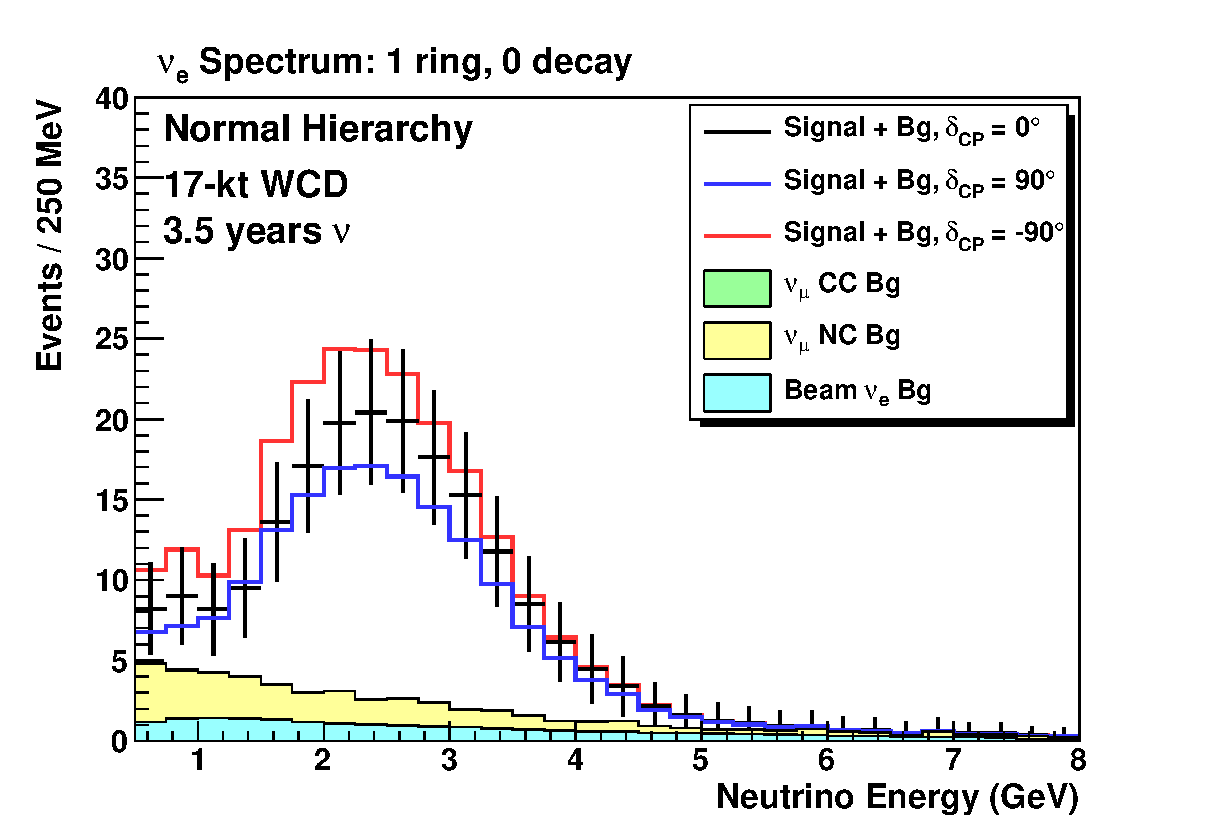
\includegraphics[width=0.3\linewidth]{lbl/nu_water_skfq_1ring0decay_normal.eps}
  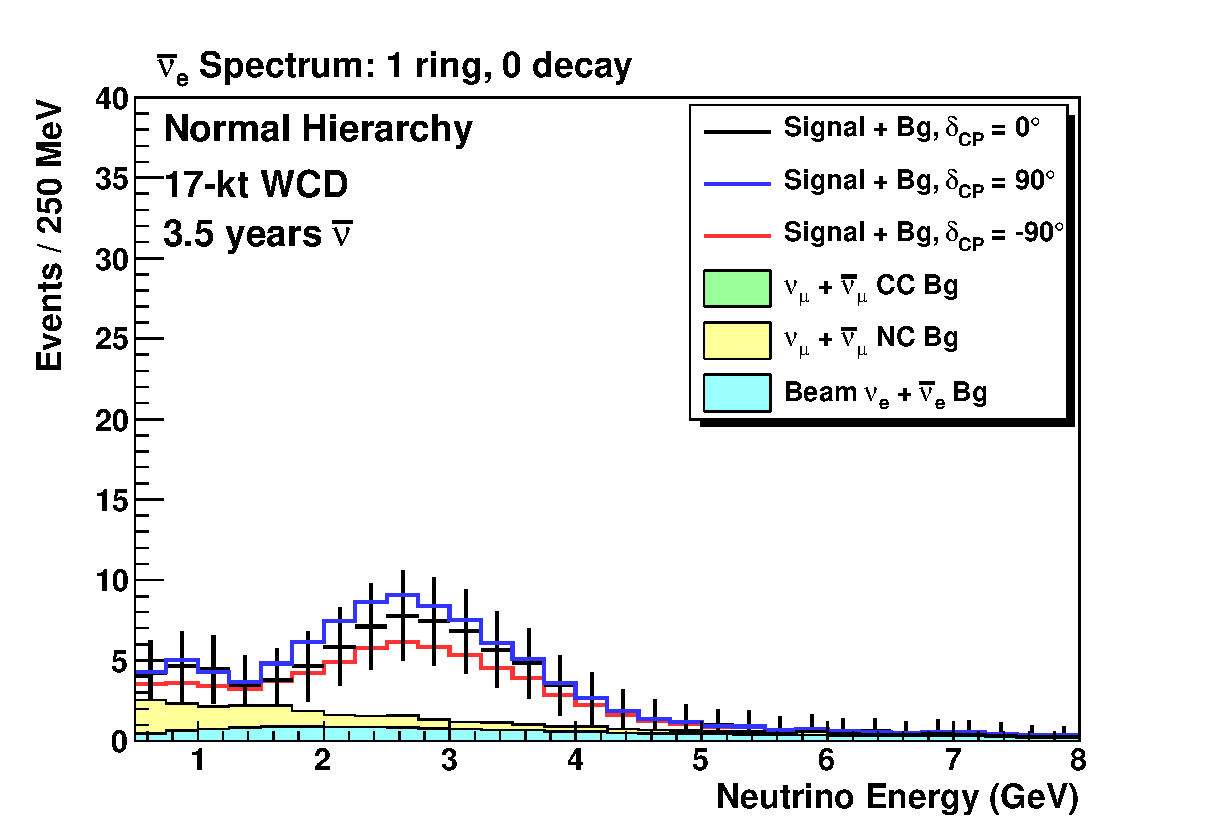
\includegraphics[width=0.3\linewidth]{lbl/anu_water_skfq_1ring0decay_normal.eps}
  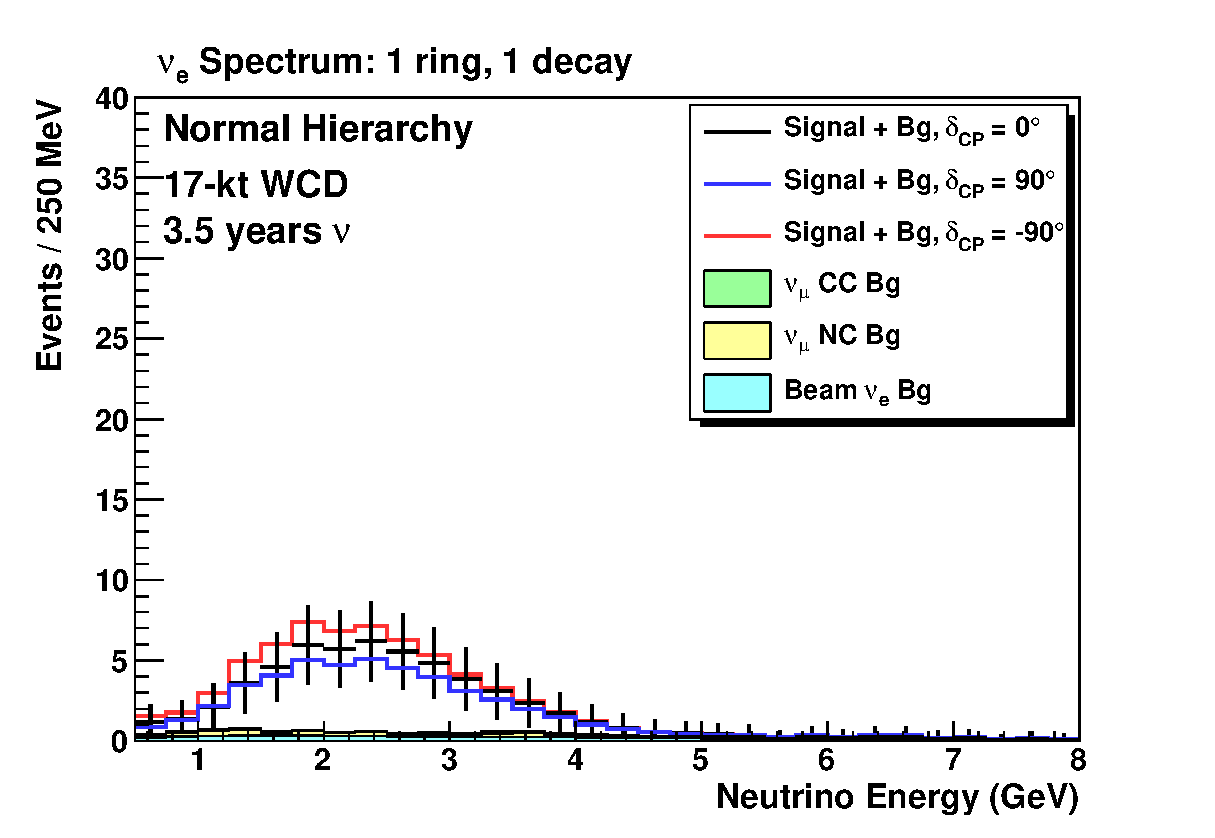
\includegraphics[width=0.3\linewidth]{lbl/nu_water_skfq_1ring1decay_normal.eps}
  \caption{Expected event rates as a function of reconstructed neutrino energy for Theia after 7 years in the LBNF beam. Left: neutrino mode 1-ring+0-decay; Middle: antineutrino mode 1-ring+0-decay; Right: neutrino mode 1-ring+1-decay. The corresponding two and three ring samples are not shown.}
  \label{fig:lblspectra}
\end{figure}

We assign independent normalization uncertainties of 2\%(5\%) on the $\nu_{e}$ and $\overline{\nu}_{e}$ appearance
signal(background). We do not explicitly include the $\nu_{\mu}$ disappearance samples, but the choice of
uncertainty for the appearance samples assumes some systematics constraint from the disappearance samples.
This treatment of systematic uncertainty is comparable to that in the DUNE CDR analysis. We find the sensitivity
of the 17-kt WCD to be comparable that of the DUNE 10-kt LArTPC, as shown in Fig.~\ref{fig:lbl17kt}.
It is expected that this will improve when the modern fast HQE PMTs, WbLS, and LAPPDs are considered. 

\begin{figure}[h!]
  \centering
  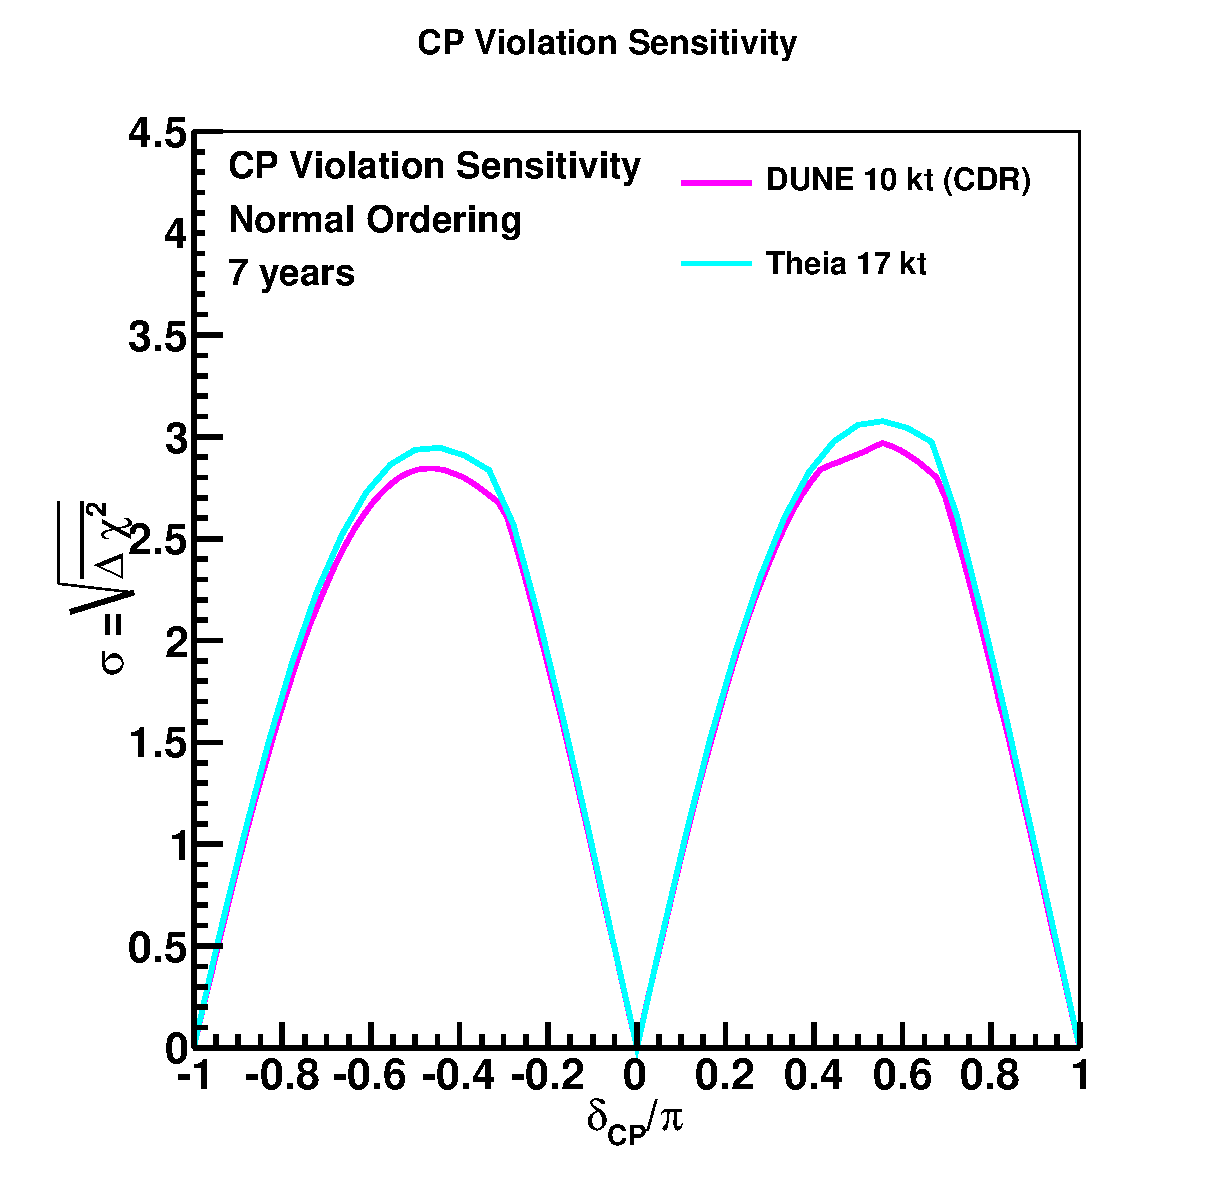
\includegraphics[width=0.45\linewidth]{lbl/cpv_theia_17kt.eps}
  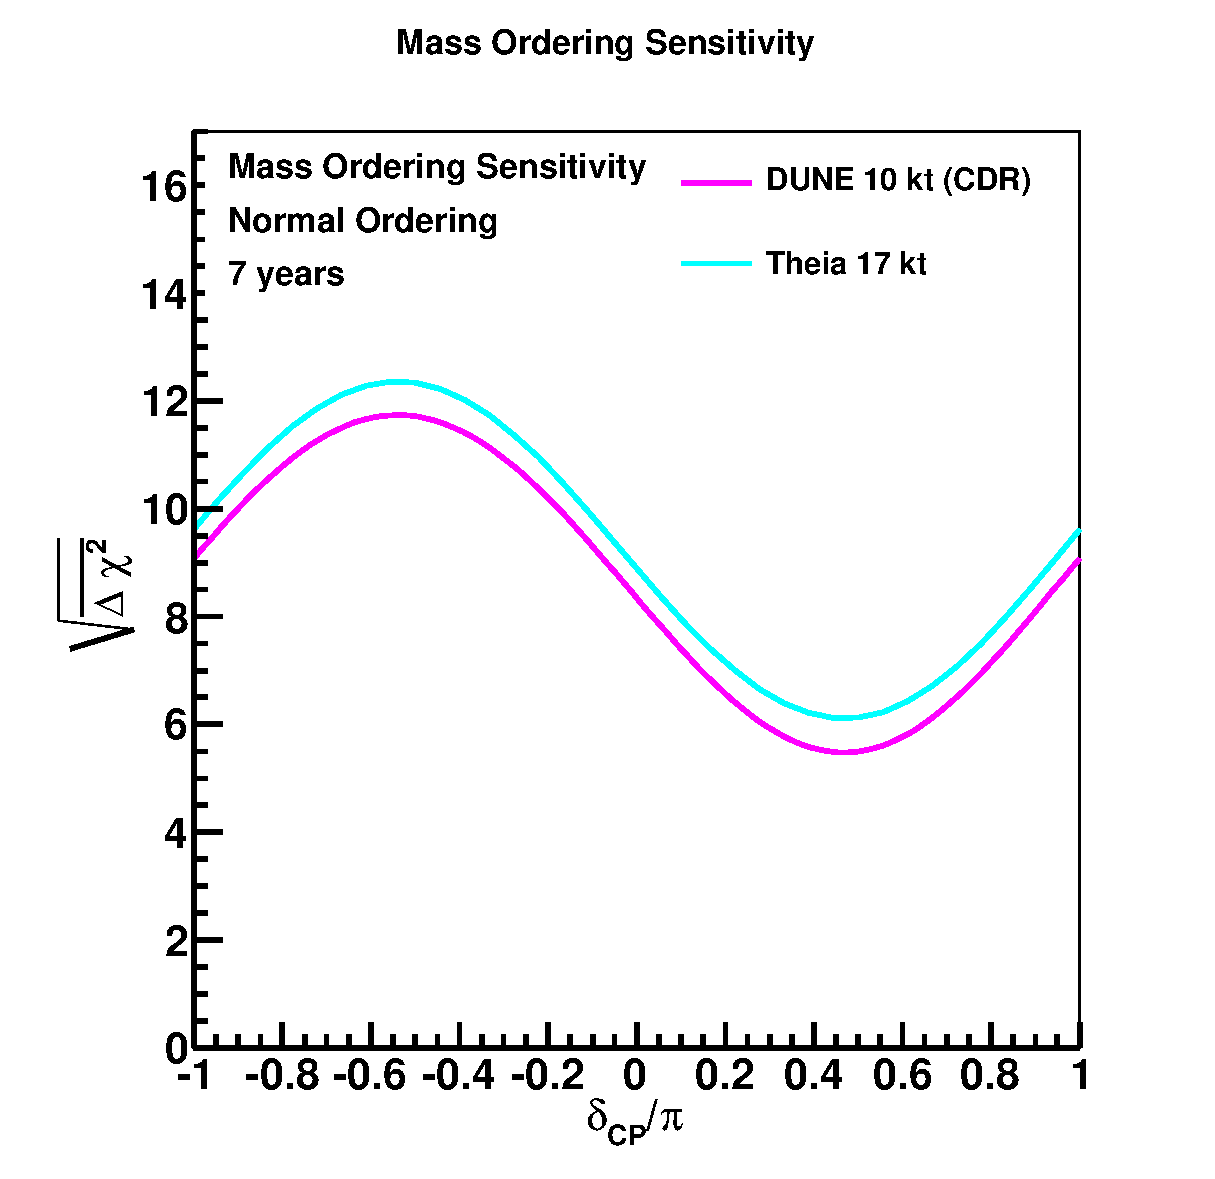
\includegraphics[width=0.45\linewidth]{lbl/mh_theia_17kt.eps}
  \caption{Sensitivity to CP violation (i.e.: determination that $\delta_{CP} \ne$ 0 or $\pi$) (left) and sensitivity
    to determination of the neutrino mass ordering (right), as a function of the true value of $\delta_{CP}$, for
    a 10-kt LArTPC (pink) compared to a 17-kt WCD (blue). Seven years of exposure to the LBNF beam
    with equal running in neutrino and antineutrino mode is assumed. LArTPC sensitivity is based on
    detector performance described by \cite{DUNEconfigs}.}
  \label{fig:lbl17kt}
\end{figure}



\subsubsection{Nucleon Decay - \bf volunteers?}
\paragraph{Motivation}
BRIEF intro to physics motivation, and status of the field: our major competitors
\paragraph{XX with THEIA}
What we bring to the table - pros of THEIA design \newline
Sensitivity estimates with baseline design (one of THEIA i--iii)
\paragraph{Detector Requirements}
A summary of the impact of different detector choices i.e. what happens if we stray from the relevant baseline
\subsubsection{Atmospheric Neutrinos - \bf volunteers?}
\paragraph{Motivation}
BRIEF intro to physics motivation, and status of the field: our major competitors
\paragraph{XX with THEIA}
What we bring to the table - pros of THEIA design \newline
Sensitivity estimates with baseline design (one of THEIA i--iii)
\paragraph{Detector Requirements}
A summary of the impact of different detector choices i.e. what happens if we stray from the relevant baseline

\subsection{Low-Energy Physics}
\subsubsection{Detector Simulation - \bf volunteers?}
Summary of simulation used in following sections, including e.g. high energy physics list, specific parameters for each detector configuration.

\input{i-DBD}
\subsection{Applied Antineutino Physics - S Dye for antinu group}
%\paragraph{Motivation}
%BRIEF intro to physics motivation, and status of the field: our major competitors
%\paragraph{XX with THEIA}
Electron antineutrinos stream freely from rapidly decaying fission products within nuclear reactors and from long-lived radioactive isotopes and their daughters within Earth \cite{agm15}. Important information about nuclear reactors, Earth, and the properties of neutrinos themselves comes from measuring the rate and energy spectrum of the interactions of these $1-10$ MeV antineutrinos. Detecting antineutrinos from nuclear reactors at short \cite{nucifer15,songs07} and long \cite{nudar13,snif10} distances monitors the operation and identifies the location and power of the reactor with applications for nuclear non-proliferation \cite{adam10}. Such detections also provide fundamental understanding of neutrinos \cite{reines53,reines76,jgl08}. Detecting antineutrinos from the nuclear cascades of thorium-232 and uranium-238 within Earth \cite{kl05} estimates terrestrial radiogenic heating \cite{gando13,agostini15}, leading to a more complete understanding of the composition, structure, and thermal evolution of our planet \cite{dye_etal15}. Global antineutrinos emerge from nuclear beta-minus decays, which produce a characteristic energy spectrum for each isotope. While the mixture of isotopes decaying within a source uniquely determines the energy spectrum of the emitted antineutrinos, neutrino oscillations distort the spectrum of detected antineutrinos in a pattern determined by the distance from the source. The rate and energy spectrum of global antineutrino interactions varies dramatically with surface location. The following discussion assumes Theia is located at SURF. Figure (surf_reac_geo.pdf) shows the energy spectrum of the predicted rate of antineutrinos at SURF.

Geo-neutrino observations probe the quantities and distributions of terrestrial heat-producing elements uranium and thorium. The quantities of these elements gauge global radiogenic power, offering insights into the origin and thermal history of the Earth. Spatial distributions reveal the initial partitioning and subsequent transport of these trace elements between metallic core, silicate mantle, and crust types. Ongoing observations at underground sites in Japan and Italy record the energies but not the directions of geo-neutrinos from uranium and thorium. Without directions pointing back to source regions, disentangling the signals from various reservoirs requires resolution of differing rates or energy spectra at separate sites. Due to limited statistics and perhaps insufficient site contrast, the observations at Japan and Italy do not yet measure distinct rates or energy spectra. Theia offers an opportunity to remedy this situation.
%What we bring to the table - pros of THEIA design \newline
%Sensitivity estimates with baseline design (one of THEIA i--iii)
%\paragraph{Detector Requirements}
%A summary of the impact of different detector choices i.e. what happens if we stray from the relevant baseline


\subsubsection{Sterile Neutrinos - \bf volunteers?}
\paragraph{Motivation}
BRIEF intro to physics motivation, and status of the field: our major competitors
\paragraph{XX with THEIA}
What we bring to the table - pros of THEIA design \newline
Sensitivity estimates with baseline design (one of THEIA i--iii)
\paragraph{Detector Requirements}
A summary of the impact of different detector choices i.e. what happens if we stray from the relevant baseline


\subsection{Astrophysical Sources}
\subsubsection{Detector Simulation}
Summary of simulation used in following sections, including e.g. high energy physics list, specific parameters for each detector configuration.

\subsection{Solar Neutrinos - GDOG, R Bonventre}
%\paragraph{Motivation}
%BRIEF intro to physics motivation, and status of the field: our major competitors
%\paragraph{XX with THEIA}
%What we bring to the table - pros of THEIA design \newline
%Sensitivity estimates with baseline design (one of THEIA i--iii)
%\paragraph{Detector Requirements}
%A summary of the impact of different detector choices i.e. what happens if we stray from the relevant baseline


Both water Cherenkov and liquid scintillator detectors have a long history of successful observation of solar neutrinos.  A number of open questions remain, including: first detection of neutrinos from the sub-dominant CNO fusion cycle, as a method to resolve the solar metallicity; a precision probe of the transition region between low-energy vacuum-dominated oscillation, below 1~MeV, and matter-dominated regime above 5~MeV, as a sensitive search for new physics effects; tests of solar luminosity through precision measurements of pep and pp neutrinos; tests of the solar temperature and, potentially, separation of the different components of the CNO flux to probe the extent to which this cycle is in equilibrium in the Sun's core.

Many of these questions can be addressed by \textsc{Theia}'s combination of a low-threshold directional detector, along with the potential for isotope loading.  \textsc{Theia} would provide unprecedented sensitivity to solar neutrinos via two channels:
\begin{enumerate}
\item {\it Huge statistics for elastic scattering (ES) events at low energy}.  
The LENA collaboration~\cite{lena} have explored in detail the power of a large-scale scintillator detector for resolving open questions in solar neutrino physics, such as determining the solar metallicity via a measurement of neutrinos from the sub-dominant CNO fusion cycle.  \textsc{Theia} would have similar capability, along with the additional advantage of being able to distinguish ES events from backgrounds (such as $^{210}$Bi) using directionality.

\item {\it Potential charged-current (CC) detection via isotope loading e.g. $^7$Li}~\cite{li}.  
The differential CC cross section for neutrino interaction on $^7$Li is extremely sharply peaked.  As a result, CC neutrino detection provides a high-precision measurement of the incoming neutrino energy, allowing extraction of the low-energy $^8$B spectrum. This would provide a sensitive search for new physics via a probe of the transition region in the neutrino spectrum between vacuum-dominated and matter-enhanced oscillations.  There is also the potential to separate the different components of the CNO flux via a shape analysis.

\end{enumerate}

\subsubsection{ES Measurements}
The sensitivity to CNO and pep solar neutrinos of an unloaded WbLS detector via the ES interaction has been studied in ~\cite{richiegdog}.  

By performing a two-dimensional  binned maximum likelihood fit  in energy and direction relative to the Sun, $\cos\theta_{\odot}$, neutrino fluxes are separated from each other, as well as  from certain sources of radioactive background.  
For each signal the $\cos\theta_{\odot}$ distribution was determined fully analytically.
All non-neutrino signals were assumed to be flat. For the solar signals the
electron direction relative to the Sun was determined
based on the differential cross sections. This was then convolved with a chosen angular resolution.  The energy response was determined semi-analytically, based on chosen detector parameters such as target light yield and photocathode coverage.  
This paper summarises the assumptions made regarding detector configuration and performance, and the resulting sensitivity to solar neutrinos. Full details of the analysis are described in~\cite{richiegdog}.  

The baseline detector configuration was chosen to be a 50-kT detector with 90\% PMT coverage, a 5\% WbLS target, and $25^\circ$ angular resolution, with baseline background levels as given in Table \ref{t:bg}. The dominant cosmogenic background, from \isotope[11]{C}, was conservatively taken to be at the Borexino level, scaled by the respective target mass.  If located at the proposed site at LBNF this background would in fact be significantly lower. All results assume a five year livetime.

\begin{table}
  {  \begin{tabular}{c c c c c}
    & H2O Level (g/gH2O) & LS Level (g/gLAB)\\
    \hline
    \isotope[238]{U} Chain & 6.63e-15 \cite{SNObg} & 1.6e-17 \cite{Borbg1}\\
    \isotope[232]{Th} Chain & 8.8e-16 \cite{SNObg} & 6.8e-18 \cite{Borbg1}\\
    \isotope[40]{K} & 6.1e-16$^a$ & 1.3e-18 \cite{Borbg2}\\
    \isotope[85]{Kr} & 2.4e-25$^b$ & 2.4e-25 \cite{Borbg2} \\
    \isotope[39]{Ar} & 2.75e-24$^b$ & 2.75e-24 \cite{Borbg2} \\
    \isotope[210]{Bi} & 3.78e-28$^b$ & 3.78e-28 \cite{Borbg2} \\
    \isotope[11]{C} & 0 & 1.0e5 (ev/kT/year) \cite{bor_be7} \\
  \end{tabular}
}
  \caption{Background assumptions for the baseline configuration. \\
  $^a$ The \isotope[40]{K} level in water is taken to be 0.1x the Borexino measurement \cite{borex_ctf}\\
  $^b$ The \isotope[85]{Kr}, \isotope[39]{Ar}, and \isotope[210]{Bi} levels in water are taken to be the Borexino measured level in scintillator \cite{Borbg2}, although levels increased by several orders of magnitude are explored \label{t:bg}
}
\end{table}

The impact of each choice of detector configuration and background level was  studied, including the target mass, the percentage loading of LS in the WbLS target, photocathode coverage, angular resolution, and background levels.  Energy reconstruction was performed semi-analytically, and the resolution was determined from a combination of the target light yield and photocathode coverage.  The effect of systematic uncertainties in both energy scale and resolution were considered.  A full reconstruction of event direction was not attempted; rather, the impact of certain values of angular resolution was considered.  In practice, the achievable angular resolution would be correlated with other detector parameters, such as the percent LS loading -- a higher fractional loading makes separation of the prompt Cherenkov signal from the isotropic scintillation more challenging, thus limiting the angular resolution.  This separation could be further enhanced by deploying fast photon sensors, such as LAPPDs~\cite{mcp--lappd3}.

The fit uncertainty for each signal with the baseline detector configuration and background assumptions is shown in Table \ref{tab:tenthk40detail}.

\begin{table}
  {  \begin{tabular}{c c c c c}
    Signal & Normalization sensitivity (\%) \\
    \hline
    \isotope[8]{B} $\nu$ & 0.4 \\
    \isotope[7]{Be} $\nu$ & 0.4 \\
    pep $\nu$ & 3.8 \\
    CNO $\nu$ & 5.3 \\
    \isotope[210]{Bi} & 0.1 \\
    \isotope[11]{C} & 11.5 \\
    \isotope[85]{Kr} & 10.5 \\
    \isotope[40]{K} & 0.04 \\
    \isotope[39]{Ar}/\isotope[210]{Po} & 21.9 \\
    \isotope[238]{U} chain & 0.02 \\
    \isotope[232]{Th} chain & 0.05 \\
  \end{tabular}}
\caption{Fit uncertainty for 5 years of data with the baseline configuration and background assumptions }
  \label{tab:tenthk40detail}
\end{table}

The impact on the CNO solar neutrino sensitivity  of detector size, LS fraction, and angular resolution for the baseline background assumptions is shown in Table \ref{tab:tenthk40} and Fig.~\ref{fig:fitresults}.

\begin{table}
 { \begin{tabular}{c c | c c c c}
      Target mass & WbLS & \multicolumn{4}{l}{Angular resolution} \\
             & & $25^\circ$ & $35^\circ$ & $45^\circ$ & $55^\circ$\\
             \hline
             50 kT & 0.5\% & 6.2 & 8.8 & 11.2 & 13.5 \\
             50 kT & 1\% & 6.1 & 8.7 & 11.0 & 13.4 \\
             50 kT & 2\% & 6.2 & 8.9 & 11.4 & 13.8 \\
             50 kT & 3\% & 5.9 & 8.4 & 10.7 & 13.0 \\
             50 kT & 4\% & 5.5 & 7.9 & 10.1 & 12.3 \\
             50 kT & 5\% & 5.3 & 7.6 & 9.7 & 11.8 \\
             \hline
             25 kT & 0.5\% & 8.5 & 12.2 & 15.6 & 18.7 \\
             25 kT & 1\% & 8.5 & 12.1 & 15.0 & 18.4 \\
             25 kT & 2\% & 8.5 & 12.1 & 15.5 & 18.7 \\
             25 kT & 3\% & 8.0 & 11.5 & 14.6 & 17.7 \\
             25 kT & 4\% & 7.6 & 10.9 & 13.9 & 16.8 \\
             25 kT & 5\% & 7.3 & 10.5 & 13.3 & 16.2 \\
  \end{tabular}}
  \caption{CNO flux sensitivity (\%) as a function of target mass, WbLS \% and angular resolution for 5 years of data with 90\% PMT coverage and the baseline background assumptions }
\label{tab:tenthk40}
\end{table}

\begin{figure}
  \includegraphics[width=3.5in]{solar/{borex01k_cno}.pdf}
  \caption{CNO sensitivity as a function of scintillator fraction and angular resolution for a 50 kT detector after 5 years of running with the baseline background assumptions \label{fig:fitresults}}
\end{figure}

A study of both energy scale and resolution systematics shows that these can be constrained by the data to sub-percent levels, making them sub-dominant in the final flux sensitivities. 

The sensitivity was shown to be extremely robust to background level variations of several orders of magnitude at the baseline angular resolution, and to the assumed level of $\beta -- \alpha$ discrimination and BiPo coincidence  rejection.  Even the dominant background to the Borexino measurement, \isotope[11]{C}, was shown to have a small impact, demonstrating that the depth of the experiment site is not a critical factor.  This is to be expected, since the directional resolution provides extremely strong separation between solar neutrino signal events and the uniform background events.  The level of $^{40}$K was observed to have the largest impact: an increase of x10 in this background reduces the CNO sensitivity by a factor of 2.  
$^{40}$K is a dominant background at
low energies. This is due to the much higher contamination in the water component of the WbLS compared to the relatively cleaner scintillator -- even assuming an order of magnitude improvement over the level measured in water by Borexino and SNO. The $^{40}$K
background in water was not critical for these previous measurements, and so it may be
possible to further reduce the level with additional effort. The SNO water
processing plant could be improved by increasing the frequency of replacing ion
exchange columns or by distilling the water. A successful measurement in WbLS would rely on such improvements.

\subsubsection{CC Measurements}

The potential for CC measurements in Theia was studied in ~\cite{asdc}.  That work is summarised here.

Several factors contribute to the choice of isotope for loading into a scintillator detector.  $^{37}$Cl and $^{71}$Ga have been used successfully by radiochemical experiments from the late 1960s to the present day.  $^{7}$Li has been considered as a favorable alternative~\cite{rcli} but such a detector was never constructed.  $^{7}$Li was also proposed as an additive to a water detector in~\cite{li}; such a detector would have excellent sensitivity to the high end of the $^8$B spectrum, but would be limited in threshold. 
As seen in Fig.~\ref{f:clga}, $^{71}$Ga and $^{7}$Li both have more favorable cross sections than $^{37}$Cl, particularly at low energies.    However, the cost of $^{71}$Ga would likely be prohibitive in a liquid scintillator experiment.  The relatively large differential uncertainties on the $^{71}$Ga cross section would also smear out any extracted spectrum whereas the cross sections on $^{37}$Cl and $^{7}$Li are known to extremely high precision.  The $^{37}$Cl cross section has been mapped using the $\beta$ decay of $^{37}$Ca.  
The CC interaction of $\nu_e$ on $^{7}$Li is shown in Eq.~(\ref{e:li}).
\begin{equation}\label{e:li}
^{7}Li + \nu_e \rightarrow\, ^{7}Be + e^- \quad \rm{(Q = 862~keV)}
\end{equation}
$^{7}$Li has only two significant transitions: a mixed Fermi and Gamow-Teller transition to the ground state of $^{7}$Be with a threshold of 0.862~MeV; and a super-allowed Gamow-Teller transition to the first excited state at $\sim$430~keV, which decays with a lifetime of $\tau \sim$200~fs.   The scattering is very hard, transferring almost all incident energy to the scattered electron.  If one could differentiate between the electron of the ground state and the $e^- + \gamma$ of the first excited state one would have a high-precision reconstruction of neutrino energy.  The two states also have precisely known angular distributions, which could then be used as an additional handle to differentiate signal from background.  Even without the use of particle ID to differentiate between states the contribution of the two is known precisely from theory, so the difference in threshold can be used to demonstrate that the two are being seen in the correct proportions.
There is also the potential to observe NC interactions on $^{7}$Li (Fig.~\ref{f:clga}), exciting the analog 478~keV first excited state of $^{7}$Li, which then decays with a lifetime of $\tau \sim$105~fs.  On preliminary investigation $^{7}$Li would thus appear to be the preferred isotope.  However, other factors may be important, such as the effect of isotope loading on scintillator optics.

\begin{figure}[!ht]
\begin{center}
\includegraphics[width=3.5in]{solar/xsecnc.pdf}
\includegraphics[width=3.5in]{solar/spectrume.pdf}
\caption{(Top) The cross section for CC neutrino interaction on $^{37}$Cl (green), $^{71}$Ga (red), and $^{7}$Li (blue) targets and NC on $^{7}$Li (blue dashed).  Data taken from~\cite{sigcl},~\cite{sigga},~\cite{sigli}, and~\cite{signc}, respectively. Although the differential uncertainties are not shown, the uncertainty on the lithium cross section is roughly 1\%~\cite{li}. (Bottom)  Predicted solar neutrino event spectra for 5 years of data-taking, with 1\% loading by mass of candidate isotopes in a 30-kT WbLS-filled ASDC detector. Solid lines show the standard solar neutrino oscillation prediction.  Dashed lines are for a flat neutrino spectrum to low energies, indicative of new physics interactions.  $^7$Li is the most favorable choice due to a high cross section for neutrino absorption.  Five years of data taking results in over 17~$\sigma$ separation in the integral flux, and correspondingly high precision (several $\sigma$ significance) on the extracted spectrum.
\label{f:clga}}
\end{center}
\vspace{-1.\baselineskip}
\end{figure}

Figure~\ref{f:solarspec} shows the predicted spectrum for the \textsc{Theia} detector assuming a 30-kT fiducial volume loaded with 1\% $^7$Li by mass, and a conservative light yield of 100 photoelectrons per MeV.  Standard MSW oscillation is assumed.  Solid lines show the CC interactions and dashed lines show ES detection.  The ES statistics by far outweigh the CC (as expected at a low \%-level loading); however, the use of directionality would allow excellent separation.  The right-hand panel shows the spectrum with a cut placed on $\cos\theta_{\odot}=0.4$ (where $\theta_{\odot}$ is the angle between the event direction and a vector pointing back to the Sun), which reduces the ES signals by more than 2 orders of magnitude.  (Angular resolution equivalent to SK-III was assumed).  In practice a more sophisticated analysis would link the normalization of the ES and CC neutrino signals via their known cross sections, allowing the ES to be used to separate events from radioactive and cosmogenic backgrounds such as $^{210}$Bi and $^{11}$C, and the CC to provide the spectral sensitivity.  The power of the CC signal can be observed in particular in the $^8$B spectrum, which has a distinctive shape, and the strong peak in the $pep$ signal in comparison to the broad ES spectrum.


\begin{figure}[!ht]
\begin{center}
\includegraphics[width=3.5in]{solar/TotalSpectrum.pdf}
\includegraphics[width=3.5in]{solar/TotalSpectrumCut.pdf}
\caption{(Top) Predicted solar neutrino spectra in a 30-kT WbLS-filled ASDC detector loaded with 1\% $^7$Li by mass.  Light yield of 100 p.e./MeV assumed.  (Bottom) The same spectra with a cut on $\cos\theta_{\odot}=0.4$, reducing the ES component to illustrate the power of CC detection.
\label{f:solarspec}}
\end{center}
\vspace{-1.\baselineskip}
\end{figure}

Due to limited sensitivity, experiments to date have only considered detection of the sum of the three CNO lines.  The increased spectral sensitivity from isotope-loaded WbLS could allow the possibility to separate the constituent lines of the CNO neutrino flux.  The CNO cycle depends critically on temperature in the conversion of C to N, reaching equilibrium only in the most central region of the solar core, where $T > 1.33\times10^7$~K.  In this region, equal numbers of neutrinos are produced in the $\beta^+$ decay of  $^{13}$N and $^{15}$O, whereas in the cooler outer regions only $^{13}$N neutrinos are produced.  Independent measurements of the $^{13}$N and $^{15}$O neutrino fluxes would determine the separate primordial abundances of C and N~\cite{HRS}.  Figure~\ref{f:cno} shows the predicted CNO spectrum broken into its individual components.  A sufficiently sensitive detector with a low enough threshold could separate the contributions from $^{13}$N and $^{15}$O.  A separate measurement of $^{17}$F is unlikely due to the much lower flux; however, there is a strong theoretical basis for fixing the $^{17}$F component to a known fraction of the sum of $^{13}$N  and $^{15}$O.

\begin{figure}[!ht]
\begin{center}
\includegraphics[width=3.5in]{solar/DetectedSpecHistCNO.pdf}
\caption{Predicted spectrum for the individual components of the CNO neutrino flux, and the total, in a WbLS detector.
\label{f:cno}}
\end{center}
\vspace{-1.\baselineskip}
\end{figure}


\subsection{Supernova Neutrinos -- Michi Wurm}

%\paragraph{Motivation}

The neutrino burst detected from the next galactic Supernova (SN) will provide us with a wealth of information on the dynamics of the core collapse (neutronization, reheating, proto-neutron star cooling) and the properties of the neutrinos themselves (mass hierarchy, absolute mass scale, collective oscillations). Since the first detection of SN neutrinos in 1987, there has been a continuous stream of new features predicted for the SN neutrino signal, hinting at new stellar or particle physics. So while we are uncertain what (superposition of) signatures to expect from the next event, it is beyond doubt that only a concerted effort of all neutrino observatories available will enable us to extract the full information contained in the burst signal, then to be combined with electromagnetic and gravitational wave observations.

If a SN neutrino burst would pass by the Earth today, the largest event statistics would be collected by the two large Cherenkov detectors, Super-Kamiokande (SK) and IceCube. Ten years from now, we may expect that additional information will be added by JUNO's liquid scintillator and DUNE's liquid argon neutrino targets. In a simplified picture, SK, JUNO and IceCube will dominate the information on $\bar\nu_e$ flux and energies, while DUNE has the potential for a high-statistics $\nu_e$ measurement. JUNO will provide information on the combined flux of $\nu_\mu$ and $\nu_\tau$ and antineutrinos (denoted commonly as $\nu_x$).

%\subsubsection{Detector Configuration}

What will THEIA add to the global picture of SN neutrino observations? To answer this, we assume a baseline detector with 50\,kt of WbLS target (10\,\% organic fraction) and 90\,\% optical coverage. The resulting photoelectron yield of $\sim$200\,p.e./MeV (75\,\% scintillation) provides a 7\,\% energy resolution comparable to present-day organic scintillator detectors and a sufficiently low threshold for high-efficiency neutron tagging.

\begin{table}[h!]
\begin{minipage}[b]{0.4\textwidth}
\begin{tabular}{llr}
\hline
\multicolumn{2}{l}{Reaction} & Rate \\
\hline
(IBD) & $\bar\nu_e+p\to n+e^+$ & 9,900 \\
(ES) & $\nu+e \to e+\nu$ & 480 \\
($\nu_e$O) & ${^{16}\rm{O}}(\nu_e,e^-){^{16}{\rm F}}$ & 170 \\
($\bar\nu_e$O) & ${^{16}\rm{O}}(\bar\nu_e,e^+){^{16}{\rm N}}$ & 220 \\
(NCO) & ${^{16}\rm{O}}(\nu,\nu){^{16}{\rm O}^*}$  & 550 \\
\hline
\end{tabular}
\caption{Event rates expected in 50\,kt of WbLS (10\,\% scintillator) for an SN at 10\,kpc distance (GVKM model \cite{Gava:2009pj} and SNOwGLoBES). We list Inverse Beta Decays (IBDs), elastic scattering off electrons (ES) as well as charged-current ($\nu_e$O,$\bar\nu_e$O) and neutral-current (NCO) interactions on oxygen. Comparatively small event rates on carbon are not listed.}
\label{tab:snrates}
\end{minipage}\hfill
\begin{minipage}[b]{0.55\textwidth}
\centering
\includegraphics[width=\textwidth]{pics/sn_spectra_new.pdf}
\captionof{figure}{Visible energy spectra of the prompt events, corresponding to the event rates of Tab.~\ref{tab:snrates} (GVKM model \cite{Gava:2009pj}). A Gaussian energy resolution of 7\,\% at 1\,MeV is applied.}
\label{fig:snspectra}
\end{minipage}
\end{table}

\begin{enumerate}
\item {\it A high-statistics and low-threshold signal:} THEIA will more than double the statistics expected for SK and JUNO in $\bar\nu_e$-induced IBD signals and add hundreds of events for $\nu_e$'s and $\nu_x$'s (Tab.~\ref{tab:snrates}). Together with a good energy resolution, this will be very useful for correlation of time-dependent spectral features with other observation techniques, e.g.~with gravitational wave emission in the early accretion phase (SASI), or when looking for energy-dependent oscillation patterns (e.g.~the spectral swaps induced by collective oscillations).
\item {\it Flavor-resolved neutrino spectra:} The presence of delayed tags from neutron capture (IBD) and re-decays of ${^{16}{\rm N}}$, the presence of $\gamma$-lines from NCO reactions  as well as the directional signature for ES will allow to resolve the integrated SN neutrino signal into its individual spectral components (Fig.~\ref{fig:snspectra}). This will enable unambiguous spectroscopy of the $\nu_e$ (ES+$\nu_e$O) and $\bar\nu_e$ (IBD+$\bar\nu_e$O) signals as well as a measurement of the combined $\nu_e+\bar\nu_e+\nu_x$ flux via NCO.
\item {\it Supernova pointing:} The presence of a high-efficiency neutron tag greatly simplifies the selection of a clean ES sample from an otherwise overwhelming IBD background \cite{Tomas:2003xn}, providing pointing accuracy on the $1^\circ$ level and thus extremely valuable information for multi-messenger observation of the early SN phases. The left panel of Fig.~\ref{fig:snpointing} exemplifies an angular distribution of directional ES and nearly isotropic IBD prompt events, assuming a tagging efficiency of 90\,\%. The right panel compares the pointing capabilities of THEIA and SK for varying assumptions on the tagging efficiency, including the upcoming SK-Gd phase.
\item {\it Neutronization burst:} While the ES signal induced by the $\nu_e$ burst from the initial phase of the core-collapse is comparatively weak, the large mass of THEIA provides $\cal O$(10) events for an SN at 10\,kpc. For a close-by SN (e.g.~1\,kpc), statistics will become sufficient to look as well for the $\nu_e$ spectrum and potential oscillation effects impacting on the burst.
\item {\it Complementarity to other observatories:} In relation to SK and JUNO, THEIA will be a further high-statistics $\bar\nu_e$ detector on the opposite of the Earth, allowing to investiagte Earth matter effects in a direct spectral comparison; regarding DUNE, THEIA will provide for a co-detection of $\nu_e$ and $\bar\nu_e$ signals in the very same location and thus information on potential differences in flavor/antiflavor oscillations for neutrinos traversing the Earth.
\end{enumerate}
 
\begin{figure}[h!]
\centering
\includegraphics[width=0.5\textwidth]{pics/sn_directionality_fit.pdf}
\hfill
\includegraphics[width=0.46\textwidth]{pics/sn_position_resolution.pdf}
\caption{SN pointing capability of THEIA, based on the reconstruction of the ES directional signal. {\it Left panel:} Example angular distribution, assuming 90\,\% in the flat IBD spectrum. Based on a fit to this and similar distributions (red net), the {\it right panel} depicts the pointing accuracy for THEIA, assuming different IBD background levels for 45\,kt as well as 22.5\,kt target mass.}
\label{fig:snpointing}
\end{figure} 
 
 
%\begin{itemize}
%\item a high-statistics and low-threshold IBD ($\bar\nu_e$) signal, offering considerably better energy resolution than SK and about twice its statistics; both aspects will prove very useful when trying to correlate spectral features changing over time with other signals, e.g.~gravitational wave emission during the SASI phase, or when looking for energy-dependent oscillation patterns (e.g.~the spectral swaps induced by collective oscillations)
%\item improved pointing accuracy for the $\nu_e$ elastic scattering signal, improving the current day $\sim$3$^\circ$ resolution of SK to the level of 1$^\circ$ or better. The key is the virtually complete subtraction of IBDs from the highly directional ES event sample that is facilitated by a high-efficiency neutron capture tag \cite{Tomas:2003xn}; SK+Gd can expect a similar improvement but offers a neutron tagging efficiency of only $\sim$70\,\%
%\item the chance to glimpse the initial $\nu_e$ neutronization burst \cite{Kachelriess:2004ds}: however, as $\cal O$(10) events are expected for a SN at 10\,kpc, detailed information can only be expected for a relatively nearby Supernova
%\item 
%\item relative to DUNE, the co-detection of $\nu_e$ and $\bar\nu_e$ signals in the very same location, allowing a direct comparison 
%\end{itemize}




%Compared to all other running and upcoming detectors (except Hyper-Kamiokande), 50\,kt of WbLS will constitute the largest neutrino target, roughly doubling the available statistics of IBDs in water (SK) and scintillator (JUNO) detectors. Moreover, THEIA will provide both good energy and directional resolution, offering handles to discriminate between different neutrino reaction channels.

%As stated above, present knowledge of the SN neutrino emission and neutrino properties does not allow for a precise prediction of the expected signal. Nevertheless, to provide a scale of the expected signal we list in table \ref{tab:snrates} the time-integrated event rates for a Supernova in 10\,kpc distance (close to the galactic center), using energies and fluxes predicted by the GVKM (Gava-Kneller-Volpe-McLaughlin) model \cite{Gava:2009pj} and the cross-sections provided by the SNOwGLoBES framework.



%\noindent {\bf Event rates.} The signal is vastly dominated by the $\bar\nu_e$-induced IBD events, followed by the NC reactions of all neutrino flavors on oxygen and elastic scattering off electrons. Note that as WbLS contains as well carbohydrates, THEIA will detect relevant numbers of neutrino events on carbon: For a 10\,\% WbLS, $\sim$250 events from NC carbon reactions are expected, inducing a gamma peak at 15\,MeV (not shown in fig.~\ref{fig:snspectra}), adding to the information on the integrated neutrino flux.
%\medskip\\
%{\bf Energy spectrum} Given its large target mass and good energy resolution, THEIA will offer detailed spectral information for the $\bar\nu_e$ flux (based on IBD events). Moreover, less precise but still relevant spectral data will be available for all other neutrino flavors that are detected in their hundreds. In figure \ref{fig:snspectra}, we show the expected event spectra as a function of their visible energy, already smeared with a 7\,\% energy resolution. As for the rate, the IBD signal dominates the interaction rates for all energies, with the noteworthy exception of the two low-energy $\gamma$ lines from the NC reaction on oxygen. However, differently from current-day water Cherenkov detectors, the neutron tag for IBD events allows to subtract the IBD signal on an event-by-event basis, providing better access for a separate study of the subdominant reaction channels. As a consequence, the gamma lines from the NC reaction are easy to extract from the remaining spectrum, providing a flavor-independent measurement of the neutrino flux \cite{Langanke:1995he,Haxton:1987kc}. Moreover, the presence of scintillation light and high energy resolution enables separate detection of the strongest gamma lines and thus a measurement of their relative spectral contributions. In case of a very efficient IBD subtraction (close to 100\,\% efficiency), there will be even some potential to separate the remaining ES, $\nu_e$O and $\bar\nu_e$O channels: ES events are strongly correlated with the SN direction and will stand out in any case (see below). Moreover, the re-decay of $^{16}$N potentially offers a delayed coincidence signature for $\bar\nu_e$O events: The remaining $\nu_e$O would then provide access to a small but pure sample of electron neutrino events. 

%\noindent{\bf Time-dependent features} A time-dependent measurement of the neutrino signal is especially interesting for studying the different phases and physical processes underlying the core collapse. For a Supernova in 10\,kpc distance, the initial neutronization burst will translate only to a small number of ES and $\nu_e$O events in THEIA, $\cal O$(10). However, if the SN were to happen closer and if the information of several detectors (especially DUNE) is combined, energy, flux and flavor content may be studied in detail. On its own, THEIA will provide detailed spectral information of the $\bar\nu_e$ flux during the accretion phase, nicely complementing the flux information available from IceCube. 
%\medskip\\
%{\bf SN neutrino pointing.} In Water Cherenkov Detectors like SK, the direction of the incoming neutrino burst can be determined based on the recoil electrons from ES: Given the relatively large neutrino energies, the electrons are very tightly aligned with the initial momentum of the neutrino. In SK, this will be sufficient to pinpoint the location of the SN within 3-4 degrees \cite{Abe:2016waf}. The most important factor limiting resolution in this case is the relatively high background formed by the only slightly directional positrons from IBD interactions. In the angular distribution of events, a peak consisting of $\sim10^2$ ES events has to be found over a flat background of several thousand IBDs.

%It has been suggested (e.g.~in \cite{Tomas:2003xn}) that the directional resolution can be considerably enhanced if the IBD events can be discriminated based on the delayed neutron tag, reducing the flat background. This represents one of the key features of SN neutrino detection in THEIA: As an example, the left panel in figure~\ref{fig:snpointing} shows the angular distribution for an SN neutrino burst (Wilson model \cite{Totani:1997vj}, 10\,kpc distance), where an efficiency of 90\,\% is assumed for IBD rejection: While the ES events are clearly peaked in the direction of the SN ($\Delta\theta=\Delta\phi=0^\circ$), the reduced IBD background constitutes only a minor background noise. 

%We studied the effect of IBD background reduction on the directional resolution based on a toy MC of the signal. For this, we fitted the output angular distribution with a radial exponential plus flat background resolution, regarding three different cases: No, 90\,\% and full IBD reduction with full detection efficiency for ES events. For the latter, we considered full event kinematics (linking electron and neutrino momentum directions) and an intrinsic angular resolution of 10$^\circ$. The results are depicted in the right panel of figure~\ref{fig:snpointing}, once for a fiducial mass of 45\,kt in the THEIA-ii configuration where close to full detection efficiency for the delayed neutron tag can be assumed, and once for half this  mass to allow for an easier comparison to current SK pointing capabilities. While we can reproduce the $\cal O$(3-4$^\circ$) pointing accuracy of SK, THEIA will reach an angular resolution of close to 1$^{\circ}$.

%It should be noted that SK+Gd will feature as well improved pointing precision based on the available delayed neutron tag. For this case, angular resolution can be estimated to $\sim$2$^{\circ}$.


\subsection{Diffuse Supernova Neutrino Background - S Dye for antinu group}
%\paragraph{Motivation}
%BRIEF intro to physics motivation, and status of the field: our major competitors
%\paragraph{XX with THEIA}
%What we bring to the table - pros of THEIA design \newline
%Sensitivity estimates with baseline design (one of THEIA i--iii)
%\paragraph{Detector Requirements}
%A summary of the impact of different detector choices i.e. what happens if we stray from the relevant baseline


\subsubsection{Indirect Dark Matter ?? }
From Michi -- there is still some interest in detecting decay/annihilation neutrinos in the multi-MeV range where THEIA would probably be able to place very competitive limits (as I noticed speaking to a theorist from Brussels a few weeks ago). It would be an addition to the antineutrino WG. Certainly, it?s rather low priority, but we could put it there as a place-holder.
\paragraph{Motivation}
BRIEF intro to physics motivation, and status of the field: our major competitors
\paragraph{XX with THEIA}
What we bring to the table - pros of THEIA design \newline
Sensitivity estimates with baseline design (one of THEIA i--iii)
\paragraph{Detector Requirements}
A summary of the impact of different detector choices i.e. what happens if we stray from the relevant baseline




%\section{Site Selection}
%
%Do we want to add this, or not really?  Maybe for the White Paper we should simply assume SURF?
%
%GDOG suggests to remove this section
%
%%\section{Baseline Detector Design}
%%\subsection{Detector Configuration Requirements}
%%Size, Depth, light yield, separation requirements
%%\subsection{WbLS Target}
%%\subsection{Photon Sensor Selection - Hybrid Scheme}
%
%\section{THEIA Timeline}
%
%Do we want to include anything on this?  Or does it simply risk that we are immediately out of date?
%
%GDOG suggests to remove this section


\section{Conclusions}

\begin{thebibliography}{00}

\bibitem{wbls}M. Yeh {\it et al.}, { ``A New Water-based Liquid Scintillator and Potential Applications.''} 
Nucl. Inst. \& Meth. A{\bf 660} 51 (2011).

\end{thebibliography}

\end{document}
